% Options for packages loaded elsewhere
\PassOptionsToPackage{unicode}{hyperref}
\PassOptionsToPackage{hyphens}{url}
%
\documentclass[
  man,floatsintext]{apa6}
\usepackage{amsmath,amssymb}
\usepackage{iftex}
\ifPDFTeX
  \usepackage[T1]{fontenc}
  \usepackage[utf8]{inputenc}
  \usepackage{textcomp} % provide euro and other symbols
\else % if luatex or xetex
  \usepackage{unicode-math} % this also loads fontspec
  \defaultfontfeatures{Scale=MatchLowercase}
  \defaultfontfeatures[\rmfamily]{Ligatures=TeX,Scale=1}
\fi
\usepackage{lmodern}
\ifPDFTeX\else
  % xetex/luatex font selection
\fi
% Use upquote if available, for straight quotes in verbatim environments
\IfFileExists{upquote.sty}{\usepackage{upquote}}{}
\IfFileExists{microtype.sty}{% use microtype if available
  \usepackage[]{microtype}
  \UseMicrotypeSet[protrusion]{basicmath} % disable protrusion for tt fonts
}{}
\makeatletter
\@ifundefined{KOMAClassName}{% if non-KOMA class
  \IfFileExists{parskip.sty}{%
    \usepackage{parskip}
  }{% else
    \setlength{\parindent}{0pt}
    \setlength{\parskip}{6pt plus 2pt minus 1pt}}
}{% if KOMA class
  \KOMAoptions{parskip=half}}
\makeatother
\usepackage{xcolor}
\usepackage{graphicx}
\makeatletter
\def\maxwidth{\ifdim\Gin@nat@width>\linewidth\linewidth\else\Gin@nat@width\fi}
\def\maxheight{\ifdim\Gin@nat@height>\textheight\textheight\else\Gin@nat@height\fi}
\makeatother
% Scale images if necessary, so that they will not overflow the page
% margins by default, and it is still possible to overwrite the defaults
% using explicit options in \includegraphics[width, height, ...]{}
\setkeys{Gin}{width=\maxwidth,height=\maxheight,keepaspectratio}
% Set default figure placement to htbp
\makeatletter
\def\fps@figure{htbp}
\makeatother
\setlength{\emergencystretch}{3em} % prevent overfull lines
\providecommand{\tightlist}{%
  \setlength{\itemsep}{0pt}\setlength{\parskip}{0pt}}
\setcounter{secnumdepth}{-\maxdimen} % remove section numbering
% Make \paragraph and \subparagraph free-standing
\makeatletter
\ifx\paragraph\undefined\else
  \let\oldparagraph\paragraph
  \renewcommand{\paragraph}{
    \@ifstar
      \xxxParagraphStar
      \xxxParagraphNoStar
  }
  \newcommand{\xxxParagraphStar}[1]{\oldparagraph*{#1}\mbox{}}
  \newcommand{\xxxParagraphNoStar}[1]{\oldparagraph{#1}\mbox{}}
\fi
\ifx\subparagraph\undefined\else
  \let\oldsubparagraph\subparagraph
  \renewcommand{\subparagraph}{
    \@ifstar
      \xxxSubParagraphStar
      \xxxSubParagraphNoStar
  }
  \newcommand{\xxxSubParagraphStar}[1]{\oldsubparagraph*{#1}\mbox{}}
  \newcommand{\xxxSubParagraphNoStar}[1]{\oldsubparagraph{#1}\mbox{}}
\fi
\makeatother
% definitions for citeproc citations
\NewDocumentCommand\citeproctext{}{}
\NewDocumentCommand\citeproc{mm}{%
  \begingroup\def\citeproctext{#2}\cite{#1}\endgroup}
\makeatletter
 % allow citations to break across lines
 \let\@cite@ofmt\@firstofone
 % avoid brackets around text for \cite:
 \def\@biblabel#1{}
 \def\@cite#1#2{{#1\if@tempswa , #2\fi}}
\makeatother
\newlength{\cslhangindent}
\setlength{\cslhangindent}{1.5em}
\newlength{\csllabelwidth}
\setlength{\csllabelwidth}{3em}
\newenvironment{CSLReferences}[2] % #1 hanging-indent, #2 entry-spacing
 {\begin{list}{}{%
  \setlength{\itemindent}{0pt}
  \setlength{\leftmargin}{0pt}
  \setlength{\parsep}{0pt}
  % turn on hanging indent if param 1 is 1
  \ifodd #1
   \setlength{\leftmargin}{\cslhangindent}
   \setlength{\itemindent}{-1\cslhangindent}
  \fi
  % set entry spacing
  \setlength{\itemsep}{#2\baselineskip}}}
 {\end{list}}
\usepackage{calc}
\newcommand{\CSLBlock}[1]{\hfill\break\parbox[t]{\linewidth}{\strut\ignorespaces#1\strut}}
\newcommand{\CSLLeftMargin}[1]{\parbox[t]{\csllabelwidth}{\strut#1\strut}}
\newcommand{\CSLRightInline}[1]{\parbox[t]{\linewidth - \csllabelwidth}{\strut#1\strut}}
\newcommand{\CSLIndent}[1]{\hspace{\cslhangindent}#1}
\ifLuaTeX
\usepackage[bidi=basic]{babel}
\else
\usepackage[bidi=default]{babel}
\fi
\babelprovide[main,import]{english}
% get rid of language-specific shorthands (see #6817):
\let\LanguageShortHands\languageshorthands
\def\languageshorthands#1{}
% Manuscript styling
\usepackage{upgreek}
\captionsetup{font=singlespacing,justification=justified}

% Table formatting
\usepackage{longtable}
\usepackage{lscape}
% \usepackage[counterclockwise]{rotating}   % Landscape page setup for large tables
\usepackage{multirow}		% Table styling
\usepackage{tabularx}		% Control Column width
\usepackage[flushleft]{threeparttable}	% Allows for three part tables with a specified notes section
\usepackage{threeparttablex}            % Lets threeparttable work with longtable

% Create new environments so endfloat can handle them
% \newenvironment{ltable}
%   {\begin{landscape}\centering\begin{threeparttable}}
%   {\end{threeparttable}\end{landscape}}
\newenvironment{lltable}{\begin{landscape}\centering\begin{ThreePartTable}}{\end{ThreePartTable}\end{landscape}}

% Enables adjusting longtable caption width to table width
% Solution found at http://golatex.de/longtable-mit-caption-so-breit-wie-die-tabelle-t15767.html
\makeatletter
\newcommand\LastLTentrywidth{1em}
\newlength\longtablewidth
\setlength{\longtablewidth}{1in}
\newcommand{\getlongtablewidth}{\begingroup \ifcsname LT@\roman{LT@tables}\endcsname \global\longtablewidth=0pt \renewcommand{\LT@entry}[2]{\global\advance\longtablewidth by ##2\relax\gdef\LastLTentrywidth{##2}}\@nameuse{LT@\roman{LT@tables}} \fi \endgroup}

% \setlength{\parindent}{0.5in}
% \setlength{\parskip}{0pt plus 0pt minus 0pt}

% Overwrite redefinition of paragraph and subparagraph by the default LaTeX template
% See https://github.com/crsh/papaja/issues/292
\makeatletter
\renewcommand{\paragraph}{\@startsection{paragraph}{4}{\parindent}%
  {0\baselineskip \@plus 0.2ex \@minus 0.2ex}%
  {-1em}%
  {\normalfont\normalsize\bfseries\itshape\typesectitle}}

\renewcommand{\subparagraph}[1]{\@startsection{subparagraph}{5}{1em}%
  {0\baselineskip \@plus 0.2ex \@minus 0.2ex}%
  {-\z@\relax}%
  {\normalfont\normalsize\itshape\hspace{\parindent}{#1}\textit{\addperi}}{\relax}}
\makeatother

\makeatletter
\usepackage{etoolbox}
\patchcmd{\maketitle}
  {\section{\normalfont\normalsize\abstractname}}
  {\section*{\normalfont\normalsize\abstractname}}
  {}{\typeout{Failed to patch abstract.}}
\patchcmd{\maketitle}
  {\section{\protect\normalfont{\@title}}}
  {\section*{\protect\normalfont{\@title}}}
  {}{\typeout{Failed to patch title.}}
\makeatother

\usepackage{xpatch}
\makeatletter
\xapptocmd\appendix
  {\xapptocmd\section
    {\addcontentsline{toc}{section}{\appendixname\ifoneappendix\else~\theappendix\fi: #1}}
    {}{\InnerPatchFailed}%
  }
{}{\PatchFailed}
\makeatother
\usepackage{csquotes}
\ifLuaTeX
  \usepackage{selnolig}  % disable illegal ligatures
\fi
\usepackage{bookmark}
\IfFileExists{xurl.sty}{\usepackage{xurl}}{} % add URL line breaks if available
\urlstyle{same}
\hypersetup{
  pdftitle={Exploring Aspects of Social Interaction using Machine Learning},
  pdfauthor={Nele-Pauline Suffo1, Pierre-Etienne Martin2, Anam Zahra2, Daniel Haun2, \& Manuel Bohn1, 2},
  pdflang={en-EN},
  hidelinks,
  pdfcreator={LaTeX via pandoc}}

\title{Exploring Aspects of Social Interaction using Machine Learning}
\author{Nele-Pauline Suffo\textsuperscript{1}, Pierre-Etienne Martin\textsuperscript{2}, Anam Zahra\textsuperscript{2}, Daniel Haun\textsuperscript{2}, \& Manuel Bohn\textsuperscript{1, 2}}
\date{}


\shorttitle{Exploring Aspects of Social Interaction using Machine Learning}

\authornote{

The authors made the following contributions. Nele-Pauline Suffo: Conceptualization, Writing - Original Draft Preparation, Writing - Review \& Editing; Manuel Bohn: Writing - Review \& Editing, Supervision.

Correspondence concerning this article should be addressed to Nele-Pauline Suffo, Universitätsallee 1, 21335 Lüneburg. E-mail: \href{mailto:nele.suffo@leuphana.de}{\nolinkurl{nele.suffo@leuphana.de}}

}

\affiliation{\vspace{0.5cm}\textsuperscript{1} Institute of Psychology in Education, Leuphana University Lüneburg\\\textsuperscript{2} Max Planck Institute for Evolutionary Anthropology}

\abstract{%
tbd
}



\begin{document}
\maketitle

\section{Introduction}\label{introduction}

\section{Methodology}\label{methodology}

The Quantex dataset includes

\subsection{Dataset Description}\label{dataset-description}

\subsubsection{Statistics}\label{statistics}

\begin{figure}

{\centering 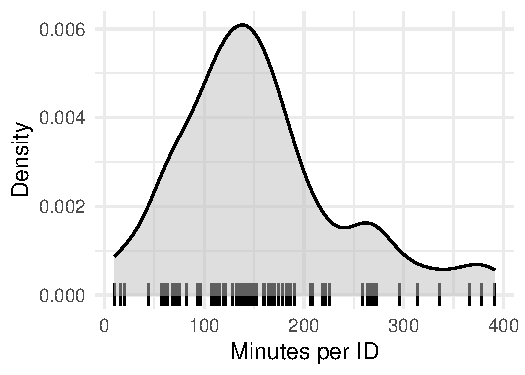
\includegraphics{Quantex_interaction_paper_files/figure-latex/quantex-minutes-per-child-1} 

}

\caption{Video recording duration (in minutes) per Child in the Quantex Dataset.}\label{fig:quantex-minutes-per-child}
\end{figure}

\subsubsection{Annotation Strategy}\label{annotation-strategy}

The dataset annotations cover four key elements: persons, faces, gaze direction, objects the child interacts with. Gaze information identifies whether a detected person's gaze is directed toward the child or not. For every detected person (or reflection of a person, such as in a mirror) and face, additional attributes like age and gender are collected. Faces are annotated even when occluded or blurry to ensure comprehensive coverage of interactions. Partially visible faces are also annotated if key facial features, such as the nose, eyes, or mouth, remain identifiable. Objects are categorized into six distinct groups: book, screen, animal, food, toy, and kitchenware, with an additional category for other objects. The dataset focus is on detecting and labeling instances of (social) interaction and engagement through these key categories. The annotation strategy is displayed in Figure \ref{fig:camera-cvat-activity-classes}.

\begin{figure}

{\centering 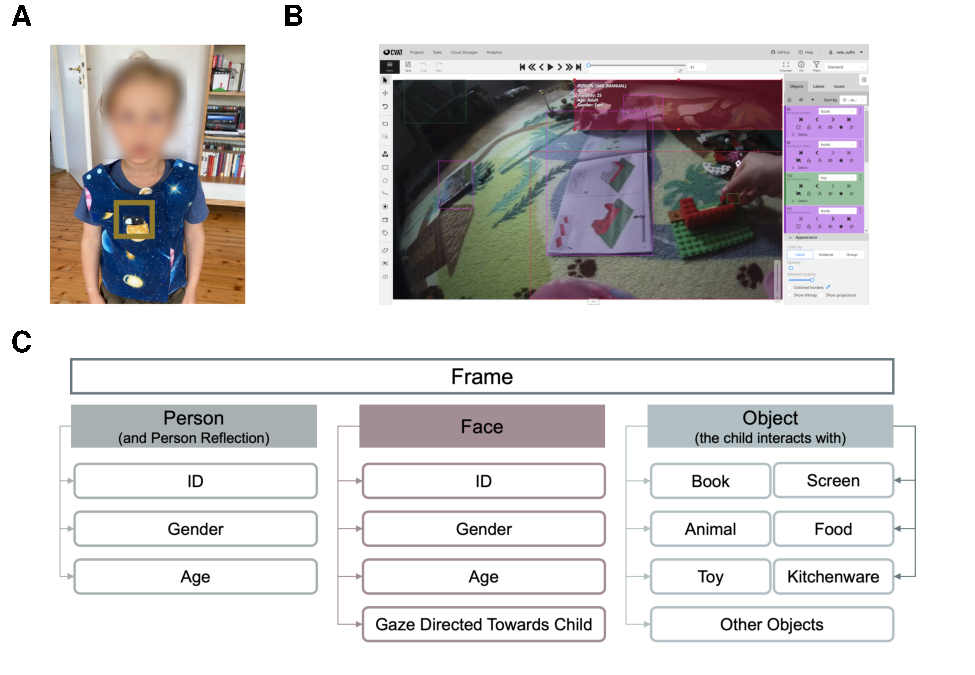
\includegraphics{Quantex_interaction_paper_files/figure-latex/camera-cvat-activity-classes-1} 

}

\caption{\textbf{A} – Vest with the embedded camera worn by the children, \textbf{B} – CVAT platform utilized for video annotation, \textbf{C} – Annotation Strategy in the Quantex dataset.}\label{fig:camera-cvat-activity-classes}
\end{figure}

\subsection{Data Collection}\label{data-collection}

This study collected egocentric video recordings from 76 children, aged 3 to 5 years, over a span of 73 months. Participating families lived in a mid-sized city in Germany. To capture the children's everyday experiences, a wearable vest equipped with a camera was used, as shown in figure \ref{fig:camera-cvat-activity-classes}. The camera, a \emph{PatrolEyes WiFi HD Infrared Police Body Camera}, provided high-definition video (1920x1080p at 30 fps) with a 140-degree wide-angle lens and also recorded audio. Children were free to move around and engage in their usual activities at home without any interference or instructions given to their parents.

\subsection{Data Preprocessing}\label{data-preprocessing}

For the video data, the annotation strategy required persons, faces, and objects to be labeled even when only partially visible, as long as key features such as facial landmarks (e.g., nose, eye, or mouth) or parts of a person or object were clearly visible. Frames that were too blurry due to movement were marked as ``noise'' and excluded from further analysis. Additionally, frames where the child was not wearing the camera, as well as any scenes containing nudity, were also labele d as noise and removed from the dataset. To prepare the video data for analysis, one frame per second was annotated, corresponding to every 30th frame in the video. Similarly, every 30th raw frame was extracted from the annotated video files. No preprocessing was applied to the audio data, which was used in its raw form for analysis.

\subsection{Automated Analysis Pipeline}\label{automated-analysis-pipeline}

\subsubsection{Person Detection}\label{person-detection}

\subsubsection{Face Detection}\label{face-detection}

\begin{table}[tbp]

\begin{center}
\begin{threeparttable}

\caption{\label{tab:face-detection-metrics}Evaluation metrics for the YOLO11 face detection model trained on the Quantex dataset.}

\begin{tabular}{llll}
\toprule
Dataset & \multicolumn{1}{c}{Precision} & \multicolumn{1}{c}{Recall} & \multicolumn{1}{c}{F1-Score}\\
\midrule
Quantex & 0.90 & 0.83 & 0.86\\
\bottomrule
\end{tabular}

\end{threeparttable}
\end{center}

\end{table}

\subsubsection{Gaze Classification}\label{gaze-classification}

\subsubsection{Voice Detection and Classification}\label{voice-detection-and-classification}

\subsection{Feature Extraction}\label{feature-extraction}

\section{Results}\label{results}

\subsection{Presence of Aspects of Social Interaction}\label{presence-of-aspects-of-social-interaction}

\subsubsection{Presence of a Person}\label{presence-of-a-person}

\subsubsection{Presence of a Face}\label{presence-of-a-face}

\subsubsection{Presence of Gaze Directed at the Child}\label{presence-of-gaze-directed-at-the-child}

\subsubsection{Presence of Language}\label{presence-of-language}

\subsection{Co-occurrence of Aspects of Social Interaction}\label{co-occurrence-of-aspects-of-social-interaction}

\section{General Discussion}\label{general-discussion}

\newpage

\section{References}\label{references}

\newpage

\section{Supplementary Material}\label{supplementary-material}

\subsection{Person Detection: Model Selection, Data Preprocessing, and Performance Evaluation}\label{person-detection-model-selection-data-preprocessing-and-performance-evaluation}

In this study, we utilized Ultralytics' YOLO11 (Jocher \& Qiu, 2024), a state-of-the-art object detection model recognized for its efficiency and accuracy. Initially, we experimented with Multi-Task Cascaded Convolutional Networks (MTCNN) face detection algorithm (Zhang, Zhang, Li, \& Qiao, 2016); however, it achieved a recall of less than 50\% on our dataset. Furthermore, the MTCNN model demands very specific picture input for fine-tuning, which is time-consuming. In contrast, YOLO11, released in October 2024, introduces new features such as the C2PSA block, which enhances spatial attention within feature maps, allowing the model to focus more precisely on critical areas of an image. Additionally, YOLO11 incorporates the C3K2 block, designed to be faster and more efficient, enhancing the overall performance of the feature aggregation process (Khanam \& Hussain, 2024). Moreover, we already had a data preparation pipeline established for YOLO11 due to its application in person detection within our project. Consequently, we selected YOLO11 for face detection and fine-tuned it on our egocentric dataset, captured using chest-mounted cameras, to adapt it to the unique characteristics of our data.

\subsubsection{Dataset Splitting and Balancing}\label{dataset-splitting-and-balancing}

We started data preprocessing with a dataset comprising a total of 113799 images from 80 annotated videos.Prior to partitioning this dataset into training, validation, and testing subsets, we analyzed the proportion of images containing annotated faces versus those without. Our analysis revealed that 45.25\% of the images included at least one annotated face. To maintain this inherent distribution across all subsets, we initially applied a stratified split, ensuring that each subset---training, validation, and testing---preserved the original 19\% to 81\% ratio of images with faces to images without faces.

However, this stratified split resulted in a significant class imbalance within the training set, which could adversely affect the model's learning process. In imbalanced datasets, models tend to be biased toward the majority class, often predicting it more frequently while misclassifying or overlooking minority class instances. This can lead to poor recall for the minority class (Hasanin, Khoshgoftaar, Leevy, \& Bauder, 2019). Additionally, Yolo11's gradient-based learning algorithm struggles to adjust decision boundaries effectively when trained on imbalanced data, potentially causing slow or unstable convergence and requiring extensive hyperparameter tuning (Kaur, Pannu, \& Malhi, 2020).

To mitigate this issue, we employed an undersampling technique on the training data. Specifically, we identified the number of images containing faces in the training set (41192 frames) and randomly sampled an equal number of images from the non-face category. This approach balanced the training dataset to consist of 50\% images with faces and 50\% images without faces, thereby addressing the class imbalance and facilitating more effective model training.

Consequently, the final data distribution was as follows: the balanced training dataset comprised 82384 frames, while the validation and test datasets contained 11379 and 11382 frames, respectively. Notably, the validation and test sets retained the original 19\% face presence, ensuring that the model's performance evaluation remained representative of the real-world data distribution.

\subsubsection{Training and Convergence}\label{training-and-convergence}

Model training was conducted on a Linux server equipped with an Intel(R) Xeon(R) Silver 4214Y CPU @ 2.20GHz with 48 cores, a Quadro RTX 8000 GPU and 188 GB of RAM. The model was trained for a total of 86 epochs. The training process utilized YOLO11's built-in data augmentation, a batch size of 16, a cosine annealing learning rate scheduler, and early stopping after 10 epochs without improvement, with a maximum of 200 epochs.

The loss function of the YOLOv11 model comprises three main components: Box Loss, Classification Loss, and Distribution Focal Loss (DFL). Box Loss estimates the difference between predicted bounding boxes and ground truth boxes to assess the model's localization accuracy. Classification Loss measures the model's ability to properly identify detected objects; however, in our study, this component is less relevant due to our focus on a single class---faces. DFL improves the model's ability to detect challenging objects by prioritizing difficult-to-detect instances.

During the training process, we observed that all three loss components decreased over time, indicating effective learning and improved performance, as visible in in figure \ref{fig:face-loss-curves}. A steady decrease in Box Loss indicates that the model is becoming increasingly accurate in localizing faces within images. This is consistent with the rapid convergence of Classification Loss, revealing the model's ability to reliably recognize faces. The decrease in DFL over time indicates that the model is getting better at focusing on and correctly identifying difficult-to-detect faces, which improves its overall detection capabilities. These data collectively represent the model's gradual improvement in both localization and identification tasks during the training period.

\begin{figure}

{\centering 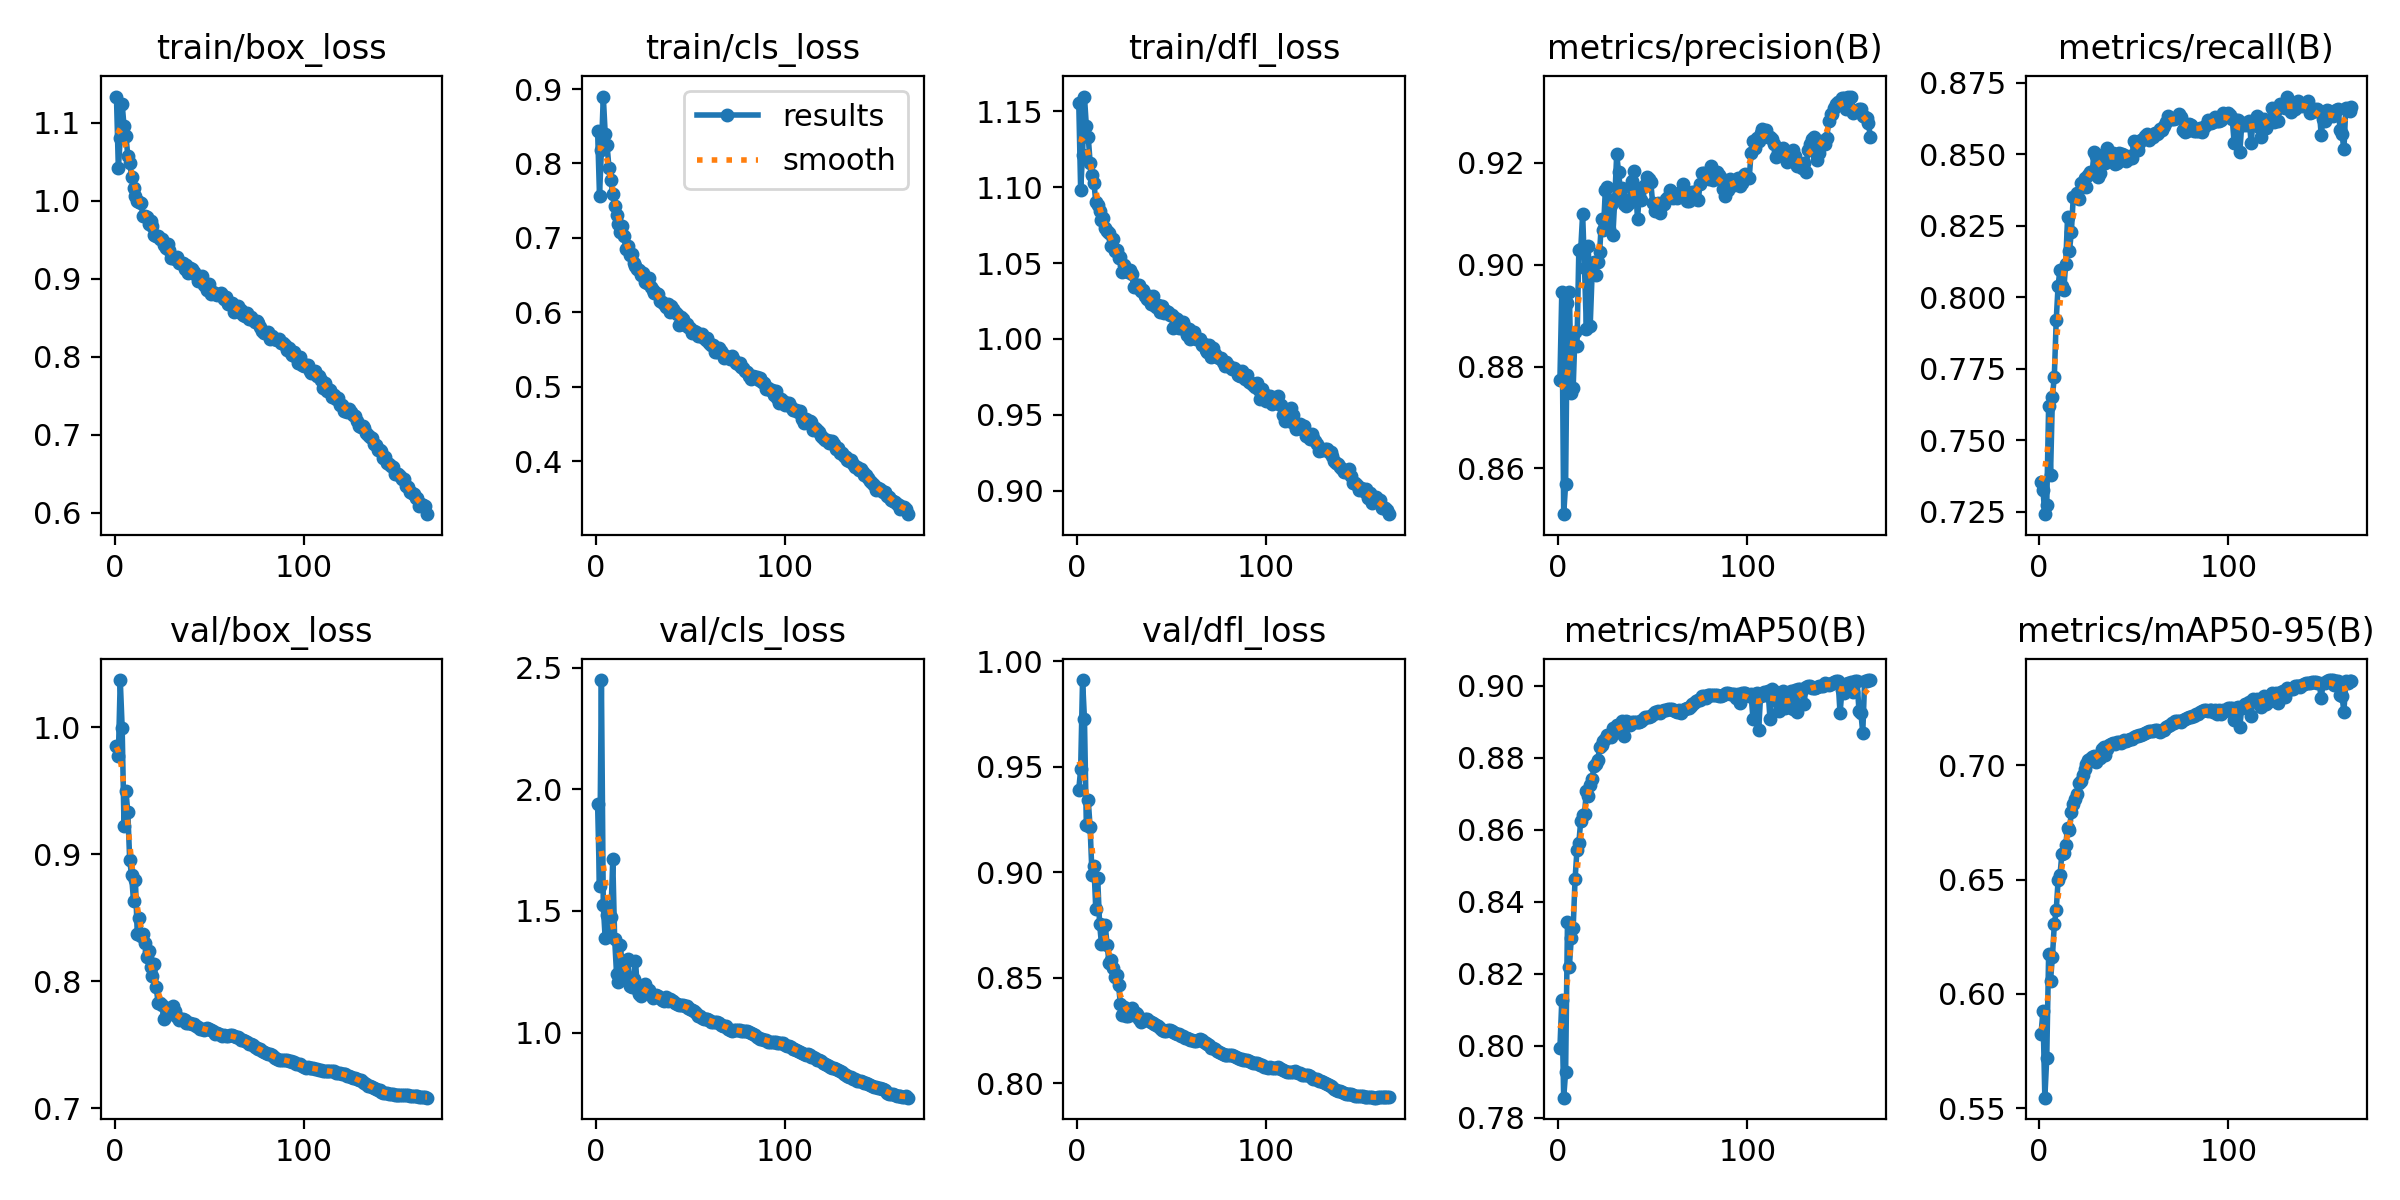
\includegraphics[width=450px]{images/yolo_face_loss_curves} 

}

\caption{Training and Validation Loss Curves for the YOLO11 face detection model.}\label{fig:person-loss-curves}
\end{figure}

\begin{table}[tbp]

\begin{center}
\begin{threeparttable}

\caption{\label{tab:person-detection-metrics-detailed}Evaluation metrics for the YOLO11 face detection model trained on the Quantex dataset. False Positive Rate and False Negative Rate are given in percentages.}

\begin{tabular}{llllll}
\toprule
Dataset & \multicolumn{1}{c}{Precision} & \multicolumn{1}{c}{Recall} & \multicolumn{1}{c}{F1-Score} & \multicolumn{1}{c}{False Positive Rate} & \multicolumn{1}{c}{False Negative Rate}\\
\midrule
Quantex & 0.90 & 0.83 & 0.86 & 2.1 & 14.0\\
\bottomrule
\end{tabular}

\end{threeparttable}
\end{center}

\end{table}

\begin{figure}

{\centering 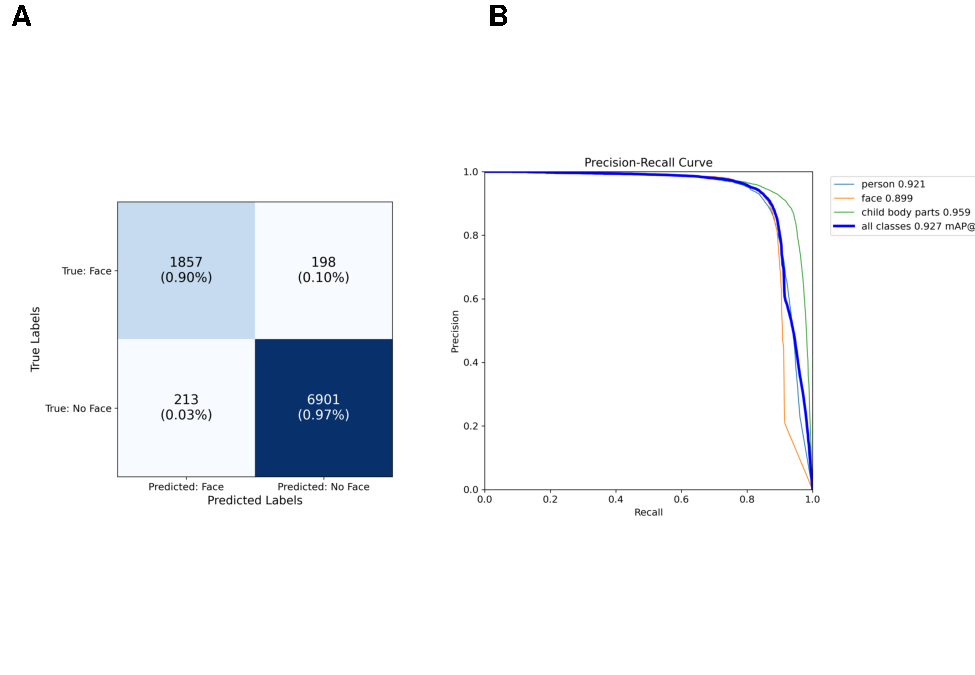
\includegraphics{Quantex_interaction_paper_files/figure-latex/person-metrics-1} 

}

\caption{\textbf{A} - Confusion Matrix for the YOLO11 face detection model trained on the Quantex dataset. \textbf{B} - Precision-Recall Curve for the YOLO11 face detection model.}\label{fig:person-metrics}
\end{figure}

\subsubsection{Model Evaluation Metrics}\label{model-evaluation-metrics}

The YOLO11 model achieved a precision of 0.92 and a recall of 0.87 on the testing set, resulting in an F1-score of 0.90. These metrics, summarized in figure \ref{fig:face-detection-metrics-detailed} indicate the model's strong performance in accurately identifying faces while minimizing errors. The precision-recall curve, displayed in figure \ref{fig:person-metrics}, further illustrates this performance, with the curve remaining close to the top-left corner. This positioning signifies that the model maintains high precision and recall across various thresholds, underscoring its effectiveness in detecting faces with confidence.

Analysis of the confusion matrix reveals that 86\% of all faces are correctly identified by the model, corresponding to 1905 true positives, while 234 faces were missed (false negatives). False negatives predominantly occurred in scenarios where faces were in the background, blurred due to motion, or occluded by the child's body. In such instances, adjacent frames often provided clearer views, aiding in more accurate classification. The model exhibited a false positive rate of approximately 2.72\%, with 251 images incorrectly classified as containing faces when none were present. These false positives were often attributed to objects or toys resembling facial features. Given the relatively low false positive rate, this small number should not raise significant concerns. In face detection systems, a balance between false positives and false negatives is often necessary, and a 2.1\% false positive rate is generally considered acceptable.

To provide a comprehensive understanding of the model's performance, we have included visual examples of true positives, false positives, and false negatives in figure \ref{fig:person-detection-examples}. These images highlight the model's strengths and areas where challenges persist, offering insights into specific scenarios that influence detection accuracy.

Overall, the YOLO11 model demonstrates robust performance in face detection tasks. However, challenges remain in dynamic scenarios, particularly with partially visible, rotated, or side-view faces. These findings underscore the complexities inherent in analyzing egocentric video data, where movement and varying perspectives introduce additional challenges.

\begin{figure}

{\centering \includegraphics{Quantex_interaction_paper_files/figure-latex/person-detection-examples-1} 

}

\caption{\textbf{A}, \textbf{B} - Examples of True Positives, \textbf{C}, \textbf{D} – Examples of False Negatives, \textbf{E}, \textbf{F} – Examples of False Positives in the YOLO11 face detection model.}\label{fig:person-detection-examples}
\end{figure}

\subsection{Face Detection: Model Selection, Data Preprocessing, and Performance Evaluation}\label{face-detection-model-selection-data-preprocessing-and-performance-evaluation}

In this study, we utilized Ultralytics' YOLO11 (Jocher \& Qiu, 2024), a state-of-the-art object detection model recognized for its efficiency and accuracy. Initially, we experimented with Multi-Task Cascaded Convolutional Networks (MTCNN) face detection algorithm (Zhang et al., 2016); however, it achieved a recall of less than 50\% on our dataset. Furthermore, the MTCNN model demands very specific picture input for fine-tuning, which is time-consuming. In contrast, YOLO11, released in October 2024, introduces new features such as the C2PSA block, which enhances spatial attention within feature maps, allowing the model to focus more precisely on critical areas of an image. Additionally, YOLO11 incorporates the C3K2 block, designed to be faster and more efficient, enhancing the overall performance of the feature aggregation process (Khanam \& Hussain, 2024). Moreover, we already had a data preparation pipeline established for YOLO11 due to its application in person detection within our project. Consequently, we selected YOLO11 for face detection and fine-tuned it on our egocentric dataset, captured using chest-mounted cameras, to adapt it to the unique characteristics of our data.

\subsubsection{Dataset Splitting and Balancing}\label{dataset-splitting-and-balancing-1}

We started data preprocessing with a dataset comprising a total of 91706 images from 64 annotated videos.Prior to partitioning this dataset into training, validation, and testing subsets, we analyzed the proportion of images containing annotated faces versus those without. Our analysis revealed that 19\% of the images included at least one annotated face. To maintain this inherent distribution across all subsets, we initially applied a stratified split, ensuring that each subset---training, validation, and testing---preserved the original 19\% to 81\% ratio of images with faces to images without faces.

However, this stratified split resulted in a significant class imbalance within the training set, which could adversely affect the model's learning process. In imbalanced datasets, models tend to be biased toward the majority class, often predicting it more frequently while misclassifying or overlooking minority class instances. This can lead to poor recall for the minority class (Hasanin et al., 2019). Additionally, Yolo11's gradient-based learning algorithm struggles to adjust decision boundaries effectively when trained on imbalanced data, potentially causing slow or unstable convergence and requiring extensive hyperparameter tuning (Kaur et al., 2020).

To mitigate this issue, we employed an undersampling technique on the training data. Specifically, we identified the number of images containing faces in the training set (13708 frames) and randomly sampled an equal number of images from the non-face category. This approach balanced the training dataset to consist of 50\% images with faces and 50\% images without faces, thereby addressing the class imbalance and facilitating more effective model training.

Consequently, the final data distribution was as follows: the balanced training dataset comprised 27416 frames, while the validation and test datasets contained 9169 and 9173 frames, respectively. Notably, the validation and test sets retained the original 19\% face presence, ensuring that the model's performance evaluation remained representative of the real-world data distribution.

\subsubsection{Training and Convergence}\label{training-and-convergence-1}

Model training was conducted on a Linux server equipped with an Intel(R) Xeon(R) Silver 4214Y CPU @ 2.20GHz with 48 cores, a Quadro RTX 8000 GPU and 188 GB of RAM. The model was trained for a total of 86 epochs. The training process utilized YOLO11's built-in data augmentation, a batch size of 16, a cosine annealing learning rate scheduler, and early stopping after 10 epochs without improvement, with a maximum of 200 epochs.

The loss function of the YOLOv11 model comprises three main components: Box Loss, Classification Loss, and Distribution Focal Loss (DFL). Box Loss estimates the difference between predicted bounding boxes and ground truth boxes to assess the model's localization accuracy. Classification Loss measures the model's ability to properly identify detected objects; however, in our study, this component is less relevant due to our focus on a single class---faces. DFL improves the model's ability to detect challenging objects by prioritizing difficult-to-detect instances.

During the training process, we observed that all three loss components decreased over time, indicating effective learning and improved performance, as visible in in figure \ref{fig:face-loss-curves}. A steady decrease in Box Loss indicates that the model is becoming increasingly accurate in localizing faces within images. This is consistent with the rapid convergence of Classification Loss, revealing the model's ability to reliably recognize faces. The decrease in DFL over time indicates that the model is getting better at focusing on and correctly identifying difficult-to-detect faces, which improves its overall detection capabilities. These data collectively represent the model's gradual improvement in both localization and identification tasks during the training period.

\begin{figure}

{\centering 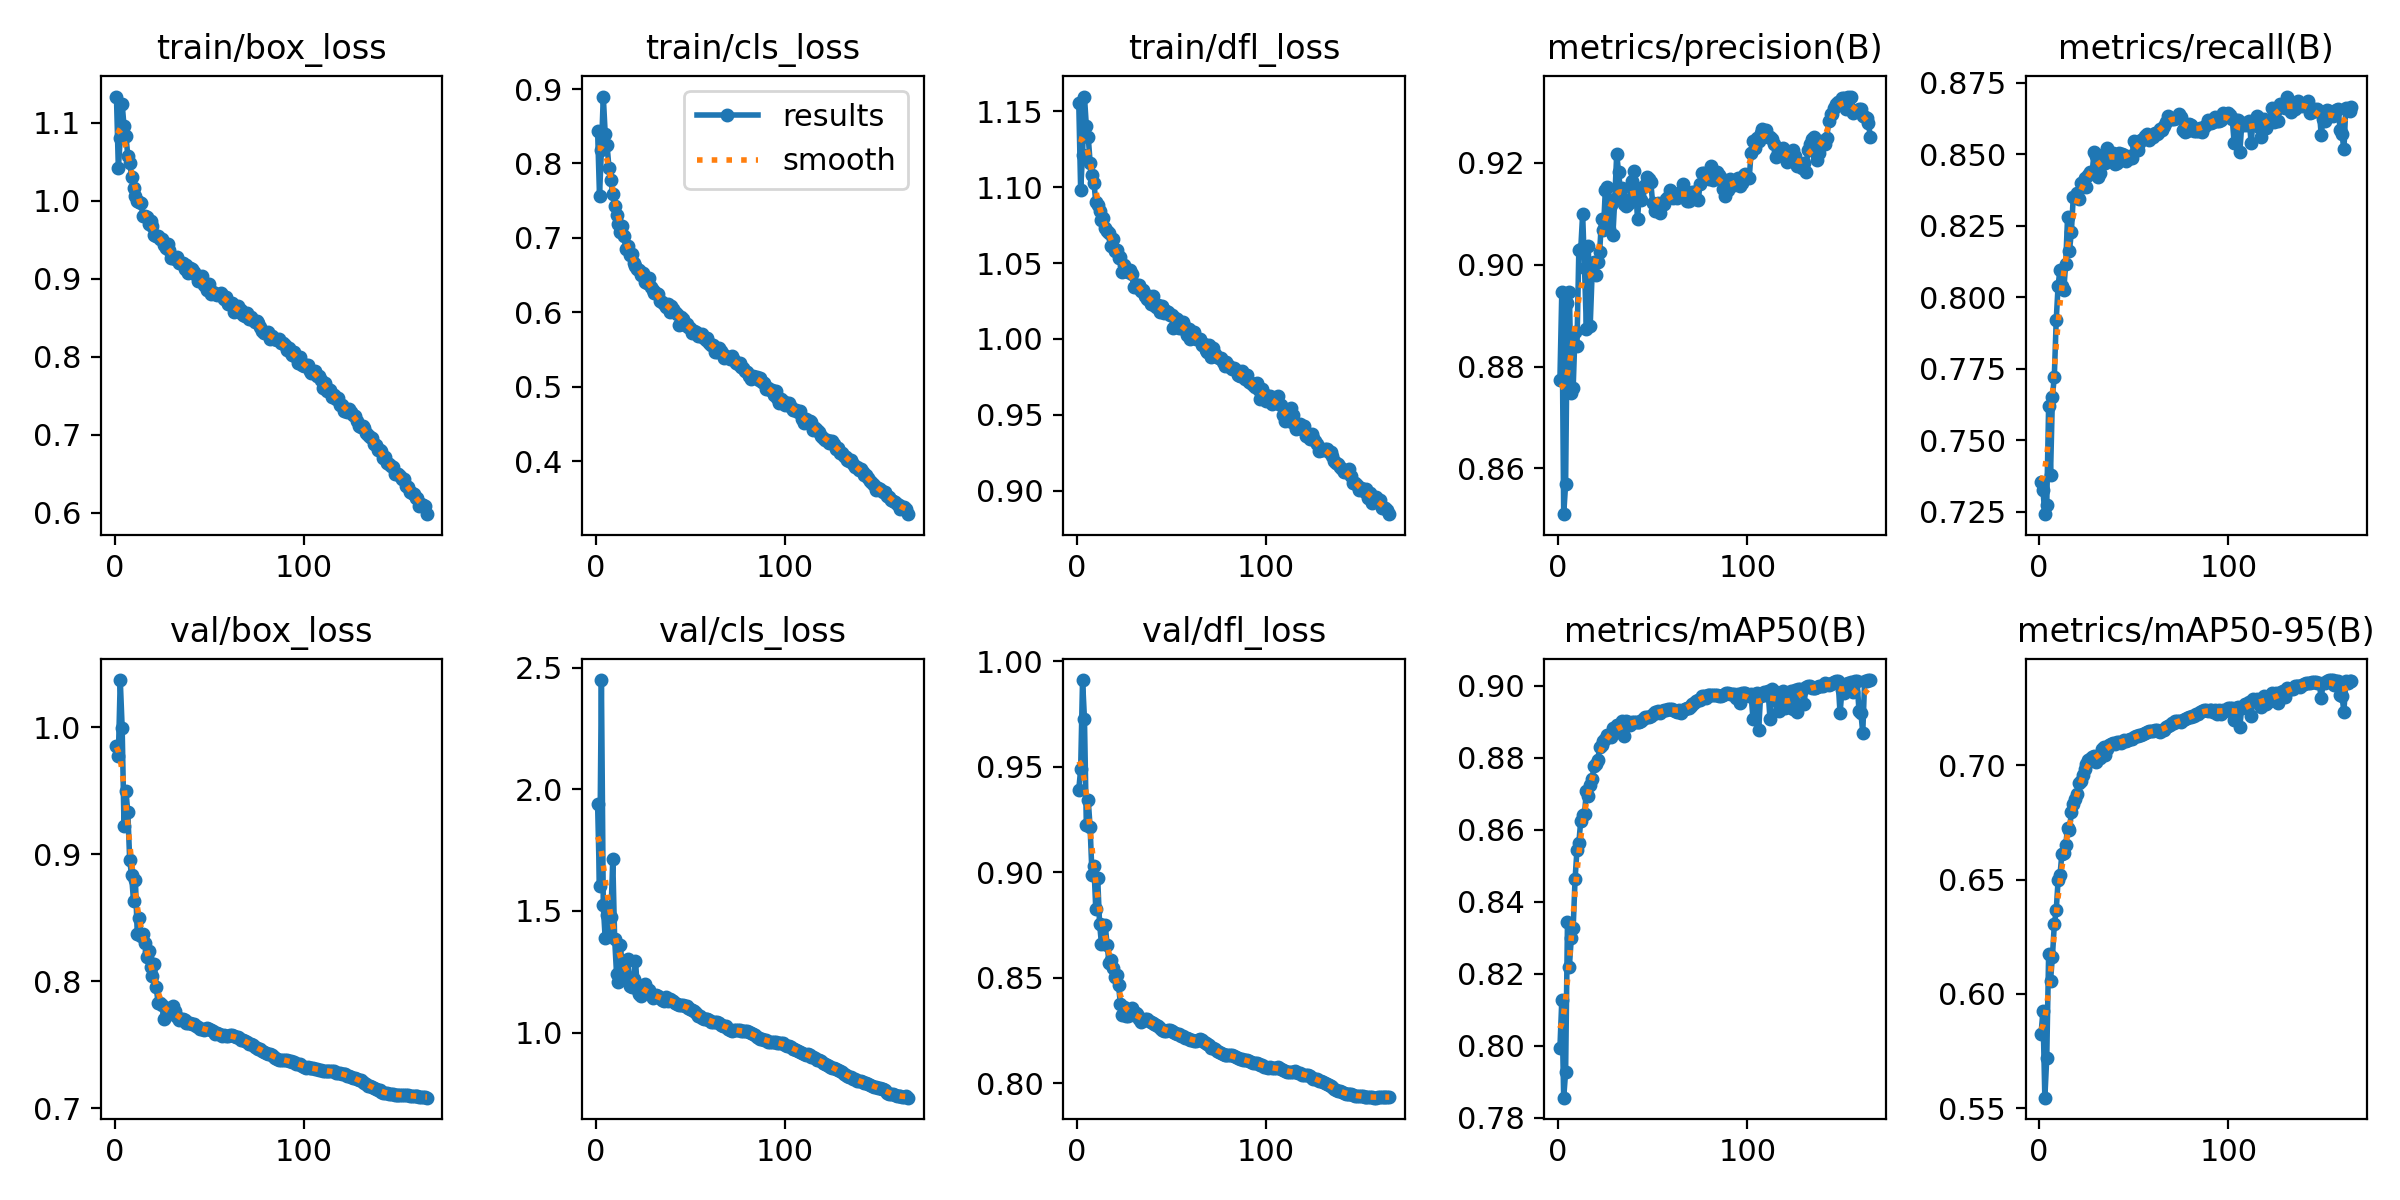
\includegraphics[width=450px]{images/yolo_face_loss_curves} 

}

\caption{Training and Validation Loss Curves for the YOLO11 face detection model.}\label{fig:face-loss-curves}
\end{figure}

\begin{table}[tbp]

\begin{center}
\begin{threeparttable}

\caption{\label{tab:face-detection-metrics-detailed}Evaluation metrics for the YOLO11 face detection model trained on the Quantex dataset. False Positive Rate and False Negative Rate are given in percentages.}

\begin{tabular}{llllll}
\toprule
Dataset & \multicolumn{1}{c}{Precision} & \multicolumn{1}{c}{Recall} & \multicolumn{1}{c}{F1-Score} & \multicolumn{1}{c}{False Positive Rate} & \multicolumn{1}{c}{False Negative Rate}\\
\midrule
Quantex & 0.90 & 0.83 & 0.86 & 2.1 & 14.0\\
\bottomrule
\end{tabular}

\end{threeparttable}
\end{center}

\end{table}

\begin{figure}

{\centering 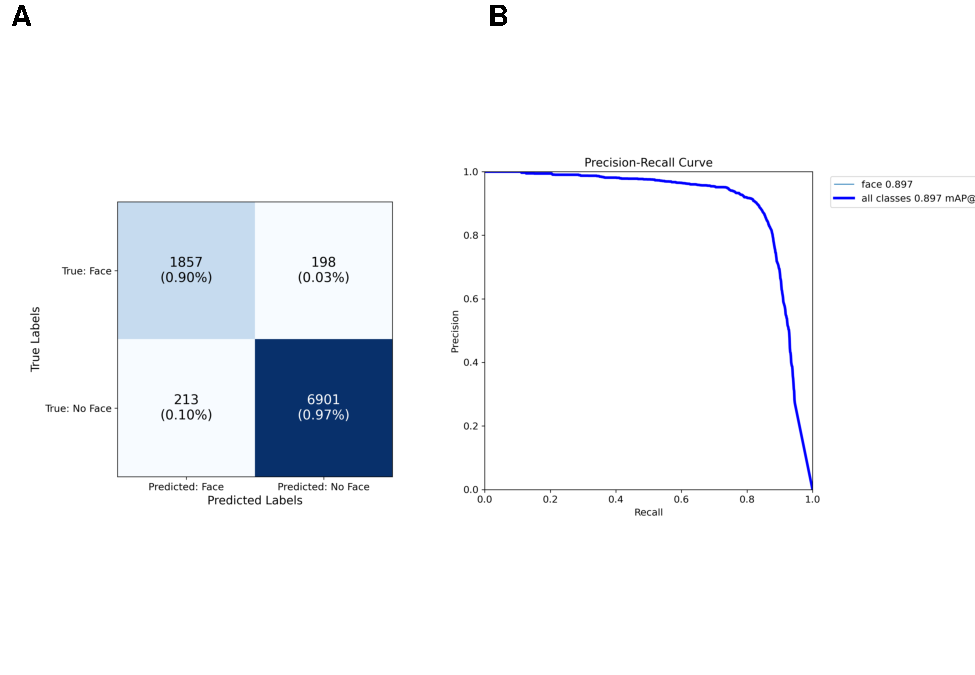
\includegraphics{Quantex_interaction_paper_files/figure-latex/face-metrics-1} 

}

\caption{\textbf{A} - Confusion Matrix for the YOLO11 face detection model trained on the Quantex dataset. \textbf{B} - Precision-Recall Curve for the YOLO11 face detection model.}\label{fig:face-metrics}
\end{figure}

\subsubsection{Model Evaluation Metrics}\label{model-evaluation-metrics-1}

The YOLO11 model achieved a precision of 0.92 and a recall of 0.87 on the testing set, resulting in an F1-score of 0.90. These metrics, summarized in figure \ref{fig:face-detection-metrics-detailed} indicate the model's strong performance in accurately identifying faces while minimizing errors. The precision-recall curve, displayed in figure \ref{fig:face-metrics}, further illustrates this performance, with the curve remaining close to the top-left corner. This positioning signifies that the model maintains high precision and recall across various thresholds, underscoring its effectiveness in detecting faces with confidence.

Analysis of the confusion matrix reveals that 86\% of all faces are correctly identified by the model, corresponding to 1905 true positives, while 234 faces were missed (false negatives). False negatives predominantly occurred in scenarios where faces were in the background, blurred due to motion, or occluded by the child's body. In such instances, adjacent frames often provided clearer views, aiding in more accurate classification. The model exhibited a false positive rate of approximately 3.57\%, with 251 images incorrectly classified as containing faces when none were present. These false positives were often attributed to objects or toys resembling facial features. Given the relatively low false positive rate, this small number should not raise significant concerns. In face detection systems, a balance between false positives and false negatives is often necessary, and a 2.1\% false positive rate is generally considered acceptable.

To provide a comprehensive understanding of the model's performance, we have included visual examples of true positives, false positives, and false negatives in figure \ref{fig:face-detection-examples}. These images highlight the model's strengths and areas where challenges persist, offering insights into specific scenarios that influence detection accuracy.

Overall, the YOLO11 model demonstrates robust performance in face detection tasks. However, challenges remain in dynamic scenarios, particularly with partially visible, rotated, or side-view faces. These findings underscore the complexities inherent in analyzing egocentric video data, where movement and varying perspectives introduce additional challenges.

\begin{figure}

{\centering \includegraphics{Quantex_interaction_paper_files/figure-latex/face-detection-examples-1} 

}

\caption{\textbf{A}, \textbf{B} - Examples of True Positives, \textbf{C}, \textbf{D} – Examples of False Negatives, \textbf{E}, \textbf{F} – Examples of False Positives in the YOLO11 face detection model.}\label{fig:face-detection-examples}
\end{figure}

\newpage

\section{References}\label{references-1}

\begingroup
\setlength{\parindent}{-0.5in}
\setlength{\leftskip}{0.5in}

\phantomsection\label{refs}
\begin{CSLReferences}{1}{0}
\bibitem[\citeproctext]{ref-hasaninSeverelyImbalancedBig2019}
Hasanin, T., Khoshgoftaar, T. M., Leevy, J. L., \& Bauder, R. A. (2019). Severely imbalanced {Big Data} challenges: Investigating data sampling approaches. \emph{Journal of Big Data}, \emph{6}(1), 107. \url{https://doi.org/10.1186/s40537-019-0274-4}

\bibitem[\citeproctext]{ref-jocherUltralyticsYOLO112024}
Jocher, G., \& Qiu, J. (2024). \emph{Ultralytics {YOLO11}}. Retrieved from \url{https://github.com/ultralytics/ultralytics}

\bibitem[\citeproctext]{ref-kaurSystematicReviewImbalanced2020}
Kaur, H., Pannu, H. S., \& Malhi, A. K. (2020). A {Systematic Review} on {Imbalanced Data Challenges} in {Machine Learning}: {Applications} and {Solutions}. \emph{ACM Computing Surveys}, \emph{52}(4), 1--36. \url{https://doi.org/10.1145/3343440}

\bibitem[\citeproctext]{ref-khanamYOLOv11OverviewKey2024}
Khanam, R., \& Hussain, M. (2024, October 23). {YOLOv11}: {An Overview} of the {Key Architectural Enhancements}. \url{https://doi.org/10.48550/arXiv.2410.17725}

\bibitem[\citeproctext]{ref-zhangJointFaceDetection2016}
Zhang, K., Zhang, Z., Li, Z., \& Qiao, Y. (2016). Joint {Face Detection} and {Alignment} using {Multi-task Cascaded Convolutional Networks}. \emph{IEEE Signal Processing Letters}, \emph{23}(10), 1499--1503. \url{https://doi.org/10.1109/LSP.2016.2603342}

\end{CSLReferences}

\endgroup

\newpage

\section{Appendix}\label{appendix}


\end{document}
